The system records which instructor teaches which course(s) in a given semester with what resources, and to enable users to answer questions about the instructors and courses.	

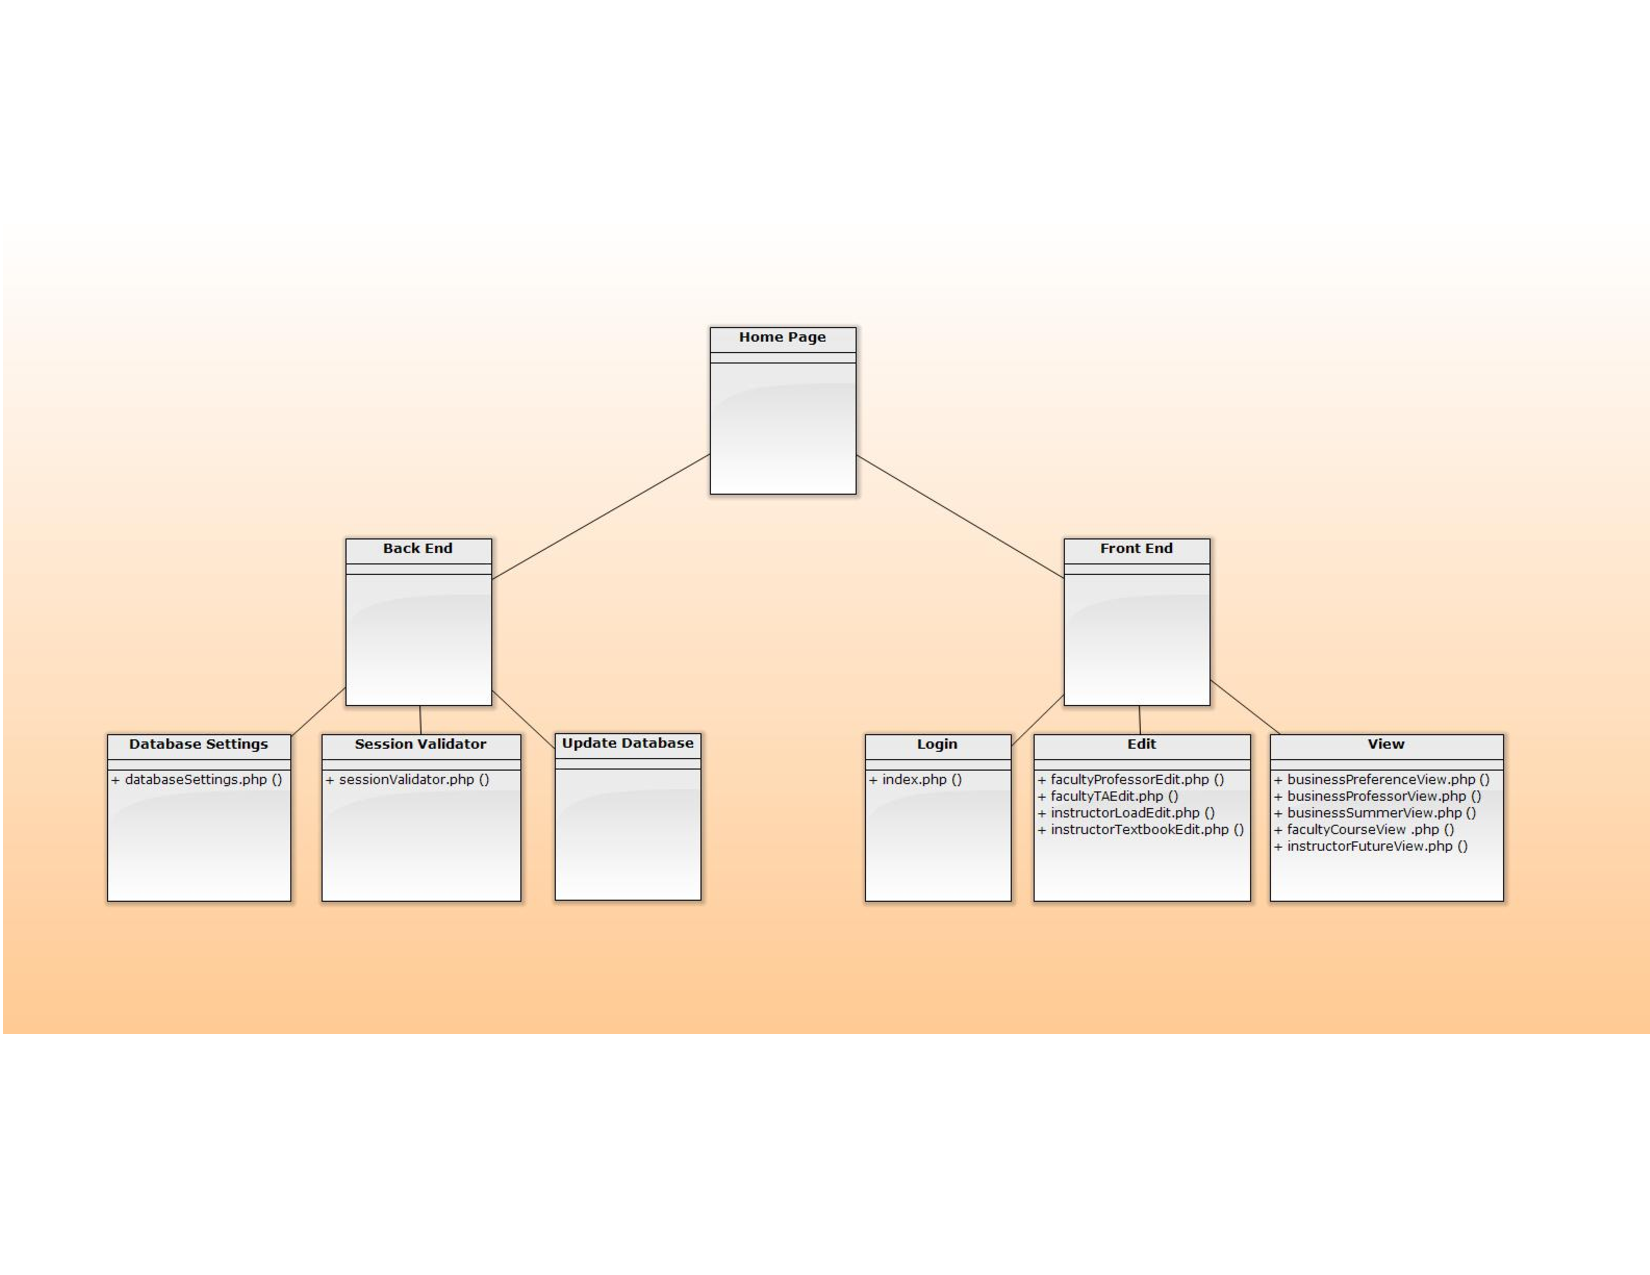
\includepdf[landscape]{design.pdf}  

%Prefers Table	

\section{Home Page}
 The home page consist of a front and back end. The front end is where the application users interact with the page directly. The back end serves indirectly in support of the front end services.
	
	\subsection{Back End}
	The back end serves indirectly in support of the front end consisting in database settings, session validation and database update applications.
	
		\subsubsection{Database Settings}
		The database settings specifies the host type, username, password, and schema for the database.
		\begin{algorithm}[H]
		\caption{Database Settings}
		\begin{algorithmic}[1]
				\State\textbf{set} host type
				\State\textbf{set} host username 
				\State\textbf{set} host password 
				\State\textbf{set} host schema
		\end{algorithmic}		 
		\end{algorithm}
		
		\subsubsection{Session Validator}
		The session validator checks the rNumber of a user after their login. 
		\begin{algorithm}[H]
		\caption{Session Validator}
		\begin{algorithmic}[1]
		\State start\_session()\Comment{PHP function creates session or resumes session}
		\If{rNumber not valid}
			\State session\_destroy()
			\State exit()
		\Else
			\If{type not valid }
			\State exit()
			\EndIf
		\EndIf
		\end{algorithmic} 
		\end{algorithm}
		
		%\subsubsection{Update Database}	
		%We need something here.
	
	\subsection{Front End}
	The front end is where the application users interact with the page directly consisting of login, edit and view applications.
		
		\subsubsection{Login}
		The login is the process by which user access to a page is controlled by identifying and authenticating the user's rNumber and password. 
		
		\begin{algorithm}[H]
			\caption{Login}
			\begin{algorithmic}[1]
			\State start\_session()
			\State \textbf{include} database settings
			\State \textbf{include} page layout
			\State \textbf{include} login box
			\If{rNumber and password}
				\State \textbf{get} int value of rNumber
				\If{rNumber $>$ 0}
				\State start connection between SQL and PHP
					\If{no connection error}
					\State \textbf{hash} password
						\If{correct password and rNumber}
					 	\State \textbf{set} expiration time for session
					 		\If{account type == faculty}
					 		\State \textbf{direct} to faculty home page 
					 		\ElsIf{account type == instructor}
					 		\State \textbf{direct} to instructor home page 
					 		\ElsIf{account type == business}
					 		\State \textbf{direct} to business home page
					 		\Else
					 		\State \textbf{diplay} error message: user has invalid account type
					 		\EndIf 	
					 	\Else
					 	\State \textbf{diplay} error message: invalid rNumber or password
					 	\EndIf 
					\Else
				 	\State \textbf{diplay} error message: invalid request
				 	\EndIf 
				\Else
			 	\State \textbf{diplay} error message: unable to connect to database	
				\EndIf
			\Else
			\State \textbf{diplay} error message: invalid rNumber	
			\EndIf			
		\end{algorithmic} 
		\end{algorithm}
		
		\subsubsection{Edit}
		
		The edit page is where the user has access to edit the data of the database according to the user's privileges. In the system a template is used to create all the edit pages, in addition each page is customized according to the system necessities. 
		
		\begin{algorithm}[H]
		\caption{Edit}
			\begin{algorithmic}[1]
			\State \textbf{set} page type to (faculty$|$instructor) 
			\State \textbf{include} database settings
			\State \textbf{include} session validator
			\State \textbf{include} page layout
			\State \textbf{open} connection with database
			\If{No connection error}
				\If{Data to display}
				\State \textbf{create} table
				\EndIf
				\While{Data to fetch}
				\State \textbf{display} data in table
				\EndWhile
			\Else
			\State \textbf{display} error message: failure to connect 
			\EndIf
			\State \textbf{get} user input data
			\State \textbf{update} database
			
			\end{algorithmic}
		\end{algorithm}
		
		\subsubsection{View}
		The view page is where the user has access to view the data of the database. In the system, a template is use to create all the view pages. In addition, each page is customized according to the system necessities. 
		
		\begin{algorithm}[H]
		\caption{View}
			\begin{algorithmic}[1]
			\State \textbf{set} page type to (faculty$|$business$|$instructor) 
			\State \textbf{include} database settings
			\State \textbf{include} session validator
			\State \textbf{include} page layout
			\State \textbf{open} connection with database
			\If{No connection error}
				\If{Data to display}
				\State \textbf{create} table
				\EndIf
				\While{Data to fetch}
				\State \textbf{display} data in table
				\EndWhile
				\State \textbf{close} connection with database
			\Else
			\State error message: failure to connect 
			\EndIf
			\end{algorithmic}
		\end{algorithm}
		
\section{General Webpage}
	\subsection{Glossary}
		\begin{itemize}
			\item AJAX: Asynchronous Javascript And XML – A way for a webpage to be updated dynamically without having to be reloaded.
			\item HTML: HyperText Markup Language – A language for describing the information contained in webpages, as well as the links between them and the visual layout/graphics.
			\item HTTP: HyperText Transfer Protocol – A standard that browsers use to send and receive information to and from web servers.
			\item Javascript – A programming language widely used within web pages, on the client side, to make them more interactive and dynamic.
			\item MySQL – A popular database system, as well as a language for retrieving and storing information in databases.
			\item PHP: PHP Hypertext Preprocessor – A programming language that resides on the server side to create dynamically generated HTML webpages.
			\item Server – A computer that hosts (stores) webpages, communicating with browsers and other entities to allow them to display the webpage's information.
			\item Web Browser – A program that connects to the internet and displays webpages.
			\item XML: eXtensible Markup Language – A language similar to HTML but more general, intended for the storage of any kind of data. Often used in conjunction with programming languages for web interaction (see AJAX)
		\end{itemize}


	\subsection{Typical Interactions with a Webpage}
		\begin{figure}[H]
			\centering
			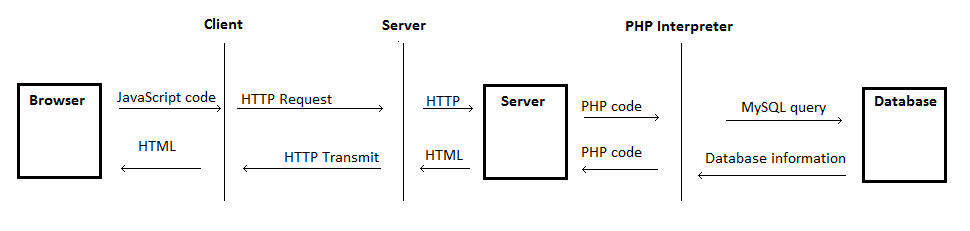
\includegraphics[scale=0.555]{Internet_Diagram.png}
			\caption{Internet Diagram}
		\end{figure}
		\begin{enumerate}
			\item A browser sends an HTTP request to a server, saying it wants the information stored in the webpages.
		
			\item 		The server receives the request. If the request is invalid a code will be transmitted that prompts the browser to display an error message.
		
			\item 		If it is valid, the server performs different operations depending on the contents of the webpage. If the page is an HTML file, it is transmitted as is. If the page is a PHP file or contains PHP code, that code is executed on the server, generating an HTML file that is sent to the user's browser (so the end user never sees the PHP code, only the HTML it generates).
		
			\item 		If the information was correctly received, the browser displays the webpage on the screen for the user to see.
		
			\item 		The user can then interact with the webpage. In our project, this mostly consists of choosing which information should be retrieved from the database and displayed – for instance, a business manager might choose which courses to display information about, or select a certain teacher from a list.

			\item 	Once the user has made a choice, they click a button (or in some other way send a request) and some Javascript code on the page is executed.
	
			\item If the page uses AJAX, the user's choices can be read and changes made to the webpage immediately, without sending a new request and reloading the page.

			\item Otherwise, their choices are transmitted to the server, once again by HTTP request. The server then can run PHP code which uses that information as input to generate HTML code based on the user's requests, which is retransmitted to their browser.

			\item Additionally, PHP code can use MySQL statements or `queries' to retrieve information from within a database on the server, and dynamically place that information into the HTML code the user receives.	

		\end{enumerate}

